\chapter{Preferred Direction Diffusion Scheme}
\label{chap:pdds}
\begin{figure}[h]
\centering
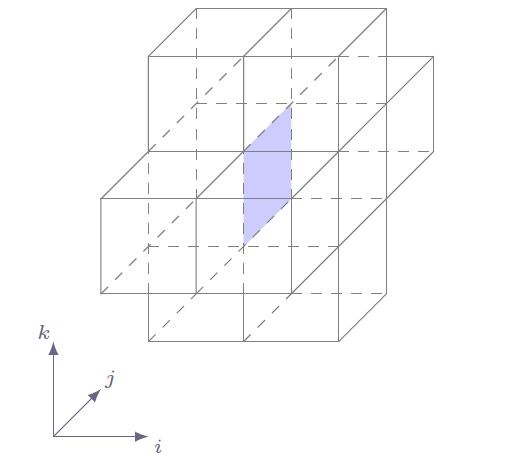
\includegraphics{figure/governing/fluxmolecule.JPG}
\caption{Representation of Flux Molecule in Computational Space}
\label{fig:fm}
\end{figure}
\hspace{0.25cm}In this new numerical scheme, the diffusion gradients on the faces are evaluated using the cell averages obtained from the surrounding ten cells as indicated in figure (\ref{fig:fm}). Note that, since the faces near domain boundaries are not surrounded by ten cells, they have to be treated differently. Twenty cell properties including volume of the cell are calculated for each of the considered ten cells per face in the physical space (\ref{sec:one}). These volume integrals are calculated using Gauss-point Quadrature (\ref{sec:gpq}).
\section{Preferred Direction}
\begin{figure}[h]
\centering
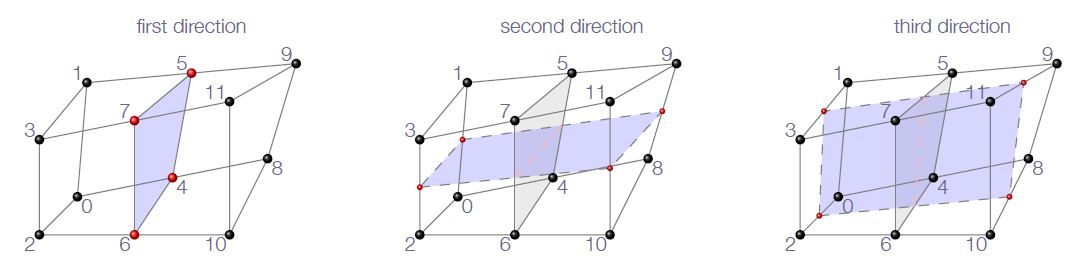
\includegraphics[width=1\linewidth]{figure/governing/pd.JPG}
\caption{Preferred Directions of a face}
\label{fig:pd}
\end{figure}
\hspace{0.25cm} In order to calculate the gradient coefficients for each face, three unique directions for each face inside the domain is calculated. Three planes are defined using the grid nodes. These directions are referred to as preferred directions, see figure (\ref{fig:pd})
      
     The preferred directions for each face of the flux molecule are calculated using the following relations,
     \begin{equation}
     \label{eq:pdeq}
         \begin{gathered}
         $First direction$,\hspace{1cm} n1=\frac{(r_7-r_4)\times(r_5-r_6)}{|(r_7-r_4)\times(r_5-r_6)|}\\
         $Second direction$,\hspace{1cm} n2=\frac{(r_{10}-r_0)\times(r_8-r_2)+(r_{11}-r_1)\times(r_9-r_3)}{|(r_{10}-r_0)\times(r_8-r_2)+(r_{11}-r_1)\times(r_9-r_3)|}\\
         $Third direction$,\hspace{1cm} n3=\frac{(r_9-r_0)\times(r_8-r_1)+(r_{11}-r_2)\times(r_{10}-r_3)}{|(r_9-r_0)\times(r_8-r_1)+(r_{11}-r_2)\times(r_{10}-r_3)|}
         \end{gathered}
     \end{equation}
The directions $n1$, $n2$ and $n3$ are not in general normal to each other.

\section{Local Co-ordinates}
    \label{sec:lc}
  \hspace{0.25cm}  A local co-ordinate system is now established for each face using the directions obtained in equation (\ref{eq:pdeq}). This co-ordinate system relates the global co-ordinate system, the preferred directions and the reference point $(x_o,y_o,z_o)$ located at the face center. 
    \begin{equation}
    \begin{gathered}
    \label{eq:lcs}
    \begin{bmatrix}
    x\\
    y\\
    z
    \end{bmatrix}= \begin{bmatrix}
    x_o\\
    y_o\\
    z_o
    \end{bmatrix}+\xi \begin{bmatrix}
    n1_x\\
    n1_y\\
    n1_z
    \end{bmatrix}+\eta\begin{bmatrix}
    n2_x\\
    n2_y\\
    n2_z
    \end{bmatrix}+\zeta\begin{bmatrix}
    n3_x\\
    n3_y\\
    n3_z\\
    \end{bmatrix}\\
    \begin{bmatrix}
    n1_x & n2_x & n3_x\\
    n1_y & n2_y & n3_y\\
    n1_z & n2_z & n3_z\\
    \end{bmatrix} 
    \begin{bmatrix}
    \xi\\
    \eta\\
    \zeta\\
    \end{bmatrix}=N\begin{bmatrix}
    \xi\\
    \eta\\
    \zeta\\
    \end{bmatrix}=\begin{bmatrix}
    x-x_o\\
    y-y_o\\
    z-z_0\\
    \end{bmatrix}\\
    \begin{bmatrix}
    \xi\\
    \eta\\
    \zeta\\
    \end{bmatrix}=N^{-1}\begin{bmatrix}
    x-x_o\\
    y-y_o\\
    z-z_0\\
    \end{bmatrix}\\
    \begin{bmatrix}
    \xi\\
    \eta\\
    \zeta\\
    \end{bmatrix}=\begin{bmatrix}
    \Psi_{11} & \Psi_{12} & \Psi_{13}\\
    \Psi_{21} & \Psi_{22} & \Psi_{23}\\
    \Psi_{31} & \Psi_{32} & \Psi_{33}\\
    \end{bmatrix}
    \begin{bmatrix}
    x-x_o\\
    y-y_o\\
    z-z_0\\
    \end{bmatrix}
    \end{gathered}
    \end{equation}
    
\section{Extraction of Gradient Coefficients}
\hspace{0.25cm}The variation of the flow variable $\varphi$ in the computational space, $(\xi,\eta,\zeta)$ is assumed to be,
\begin{equation}\label{eq:nmnm}
    {\varphi}(\xi,\eta,\zeta)=C_0+C_1\xi+C_2\eta+C_3\zeta+C_4\xi\eta+C_5\xi\zeta+C_6\eta^2+C_7\zeta^2+C_8\xi\eta^2+C_9\xi\zeta^2
\end{equation}

The unknown coefficients $[C_0....C_9]$ are obtained by solving a system of equations obtained by integrating the equation (\ref{eq:nmnm}) over the ten cell volumes of a Flux molecule (see figure \ref{fig:fm}).

\begin{equation}
\label{eq:big}
\begin{gathered}
    \begin{bmatrix}
    \overline{\varphi}_0 V_0 &.&.&.&
    \overline{\varphi}_9 V_9 
    \end{bmatrix}=\begin{bmatrix}
    C_0 &.&.&.&
    C_9
    \end{bmatrix}\begin{bmatrix}
    \int\int\int_{\Omega_0}\,d\Omega& \cdots \int\int\int_{\Omega_0} \xi\zeta^2 d\,\Omega \\
    .   &                                                                        .\\
    .    &                                                                        .\\
    .     &                                                                          .\\
    \int\int\int_{\Omega_9}\,d\Omega& \cdots \int\int\int_{\Omega_9} \xi\zeta^2 d\,\Omega \\
    \end{bmatrix}\\
    $Or$\\
    {\Phi}=\begin{bmatrix}
    C_0 &.&.&.&
    C_9
    \end{bmatrix} A
    \end{gathered}
\end{equation}
In equation (\ref{eq:big}), $\Phi$ represents the degrees of freedom in the CFD solver (cell-averages of the considered solver variables). Since the vector $\Phi$ is known the matrix $A$ can be calculated from the known metric data obtained in equations (\ref{eq:eqns} and \ref{eq:lcs}). Thus, the vector $\Phi$ can be represented as,
\begin{equation}
    \begin{bmatrix}
    C_0&.&.&.&C_9
    \end{bmatrix}=\Phi A^{-1}
\end{equation}
A detailed derivation of the integrals in the $A$ matrix is provided in Appendix \ref{app:aa}. Also, the procedure for obtaining the integrals in the domain boundaries is provided.

\section{Face Gradients}
\hspace{0.25cm}Further, differentiating equation (\ref{eq:nmnm}),
\begin{equation}
\label{eq:a18}
\begin{gathered}
    {d\varphi}=C_1d\xi+C_2d\eta+C_3d\zeta+C_4\xi d\eta+C_4\eta d\xi+C_5 \xi d\zeta+C_5 \zeta d\xi+\\
    2C_6\eta d\eta+2C_7\zeta d\zeta+C_8 \xi \eta d\eta+C_8 \eta^2 d\xi+2C_9\xi\zeta d\zeta+C_9\zeta^2 d\xi
\end{gathered}
\end{equation}
Since the local coordinate system is centered at the face center, equation (\ref{eq:a18}) results in,
\begin{equation}
    \label{eq:a19}
    \begin{gathered}
    (\xi,\eta,\zeta)=(0,0,0)\\
    {d\varphi}=C_1d\xi+C_2d\eta+C_3d\zeta
    \end{gathered}
\end{equation}
By Differentiating the second equation in (\ref{eq:lcs}), the relationship between the derivatives in ($x$,$y$,$z$) space and ($\xi$,$\eta$,$\zeta$) space is obtained as,
\begin{equation}
    \label{eq:a20}
    \begin{gathered}
    \begin{bmatrix}
    dx\\
    dy\\
    dz\\
    \end{bmatrix}=\begin{bmatrix}
    n1_x&n2_x&n3_x\\
    n1_y&n2_y&n3_y\\
    n1_z&n2_z&n3_z\\
    \end{bmatrix} \begin{bmatrix}
    d\xi\\
    d\eta\\
    d\zeta\\
    \end{bmatrix}=N \begin{bmatrix}
     d\xi\\
    d\eta\\
    d\zeta\\
    \end{bmatrix}
    \end{gathered} 
\end{equation}
Finally, the equations in (\ref{eq:a19} and \ref{eq:a20}) are combined to obtain the coefficients required for calculating the derivatives of ${\varphi}$ in the Cartesian coordinate system ($x$,$y$,$z$) at the face center.
\begin{equation}
    \label{eq:a21}
    \begin{gathered}
    \begin{bmatrix}
    Cx_0\\
    .\\
    .\\
    .\\
    Cx_9\\ \end{bmatrix}= \begin{bmatrix}
    (n1_xA^{-1}_{10}+n2_xA^{-1}_{20}+n3_xA^{-1}_{30})V_0\\
    \cdot\\
    \cdot\\
    \cdot\\
    (n1_xA^{-1}_{19}+n2_xA^{-1}_{29}+n3_xA^{-1}_{39})V_9\\
    \end{bmatrix}\\
     \begin{bmatrix}
    Cy_0\\
    .\\
    .\\
    .\\
    Cy_9\\ \end{bmatrix}= \begin{bmatrix}
    (n1_yA^{-1}_{10}+n2_yA^{-1}_{20}+n3_yA^{-1}_{30})V_0\\
    \cdot\\
    \cdot\\
    \cdot\\
    (n1_yA^{-1}_{19}+n2_yA^{-1}_{29}+n3_yA^{-1}_{39})V_9\\
    \end{bmatrix}\\
     \begin{bmatrix}
    Cz_0\\
    .\\
    .\\
    .\\
    Cz_9\\ \end{bmatrix}= \begin{bmatrix}
    (n1_zA^{-1}_{10}+n2_zA^{-1}_{20}+n3_zA^{-1}_{30})V_0\\
    \cdot\\
    \cdot\\
    \cdot\\
    (n1_zA^{-1}_{19}+n2_zA^{-1}_{29}+n3_zA^{-1}_{39})V_9\\
    \end{bmatrix}\\
    \\
    \\
     \frac{\partial {\varphi}}{\partial x} = \begin{bmatrix}
    Cx_0....Cx_9
    \end{bmatrix} \begin{bmatrix}
    \overline{{\varphi}_0}\\
   \cdot\\
    \cdot\\
    \cdot\\
    \overline{{\varphi}_9}
    \end{bmatrix},
    \frac{\partial {\varphi}}{\partial y} = \begin{bmatrix}
    Cy_0....Cy_9
    \end{bmatrix} \begin{bmatrix}
    \overline{{\varphi}_0}\\
    \cdot\\
    \cdot\\
    \cdot\\
    \overline{{\varphi}_9}
    \end{bmatrix},
    \frac{\partial {\varphi}}{\partial z} = \begin{bmatrix}
    Cz_0....Cz_9
    \end{bmatrix} \begin{bmatrix}
    \overline{{\varphi}_0}\\
   \cdot\\
    \cdot\\
    \cdot\\
    \overline{{\varphi}_9}
    \end{bmatrix}
    \end{gathered}
\end{equation}


